\RequirePackage{plautopatch} % automatically load (u)pLaTeX patched version package.
\documentclass[
  10pt,      % 10 pt
  a4j,       % A4 small margin
  twocolumn, % 2-column
  % english,   % Uncomment if you are writing the manuscript in English.
  uplatex,
  dvipdfmx
]{jsarticle}
% load IML style file.
\usepackage[smartref]{iml_resume}

%%% load packages
\usepackage{bm}
%%%

%%%% header
\LeftHeader{2023年度 卒業論文発表会(2023年11月21日)}
\makeheader
%%%%


\title{ぞうの卵のぞうの卵によるぞうの卵ためのぞうの卵 \linebreak 象卵の象卵による象卵ための象卵}
\author{姓 名}

\begin{document}

\maketitle

\section{はじめに}
\label{sec:introduction}
ぞうの卵はおいしいぞう\footnote{あくまで個人の感想です.}.ぞうの卵はおいしいぞう.ぞうの卵はおいしいぞう.ぞうの卵はおいしいぞう.ぞうの卵はおいしいぞう.ぞうの卵はおいしいぞう.ぞうの卵はおいしいぞう.ぞうの卵はおいしいぞう.ぞうの卵はおいしいぞう.ぞうの卵はおいしいぞう.ぞうの卵はおいしいぞう.ぞうの卵はおいしいぞう.ぞうの卵はおいしいぞう.ぞうの卵はおいしいぞう.ぞうの卵はおいしいぞう.ぞうの卵はおいしいぞう.ぞうの卵はおいしいぞう.ぞうの卵はおいしいぞう.ぞうの卵はおいしいぞう.ぞうの卵はおいしいぞう.ぞうの卵はおいしいぞう.ぞうの卵はおいしいぞう.ぞうの卵はおいしいぞう.ぞうの卵はおいしいぞう.ぞうの卵はおいしいぞう.ぞうの卵はおいしいぞう.ぞうの卵はおいしいぞう.ぞうの卵はおいしいぞう.ぞうの卵はおいしいぞう.ぞうの卵はおいしいぞう.ぞうの卵はおいしいぞう.ぞうの卵はおいしいぞう.ぞうの卵はおいしいぞう.ぞうの卵はおいしいぞう.ぞうの卵はおいしいぞう.ぞうの卵はおいしいぞう.ぞうの卵はおいしいぞう.ぞうの卵はおいしいぞう.ぞうの卵はおいしいぞう.ぞうの卵はおいしいぞう.ぞうの卵はおいしいぞう.ぞうの卵はおいしいぞう.ぞうの卵はおいしいぞう.ぞうの卵はおいしいぞう.ぞうの卵はおいしいぞう.ぞうの卵はおいしいぞう.ぞうの卵はおいしいぞう.ぞうの卵はおいしいぞう.ぞうの卵はおいしいぞう.ぞうの卵はおいしいぞう.ぞうの卵はおいしいぞう.ぞうの卵はおいしいぞう.ぞうの卵はおいしいぞう.ぞうの卵はおいしいぞう.ぞうの卵はおいしいぞう.ぞうの卵はおいしいぞう.ぞうの卵はおいしいぞう.ぞうの卵はおいしいぞう.ぞうの卵はおいしいぞう.ぞうの卵はおいしいぞう.ぞうの卵はおいしいぞう.ぞうの卵はおいしいぞう.ぞうの卵はおいしいぞう.ぞうの卵はおいしいぞう.ぞうの卵はおいしいぞう.ぞうの卵はおいしいぞう.ぞうの卵はおいしいぞう.ぞうの卵はおいしいぞう.

\subsection{そして}
ぞうの卵はおいしいぞう.ぞうの卵はおいしいぞう.ぞうの卵はおいしいぞう.ぞうの卵はおいしいぞう.ぞうの卵はおいしいぞう.ぞうの卵はおいしいぞう.ぞうの卵はおいしいぞう.ぞうの卵はおいしいぞう.ぞうの卵はおいしいぞう.ぞうの卵はおいしいぞう.ぞうの卵はおいしいぞう.ぞうの卵はおいしいぞう.ぞうの卵はおいしいぞう.ぞうの卵はおいしいぞう.ぞうの卵はおいしいぞう.ぞうの卵はおいしいぞう.ぞうの卵はおいしいぞう.ぞうの卵はおいしいぞう.ぞうの卵はおいしいぞう.ぞうの卵はおいしいぞう.ぞうの卵はおいしいぞう.ぞうの卵はおいしいぞう.ぞうの卵はおいしいぞう.ぞうの卵はおいしいぞう.ぞうの卵はおいしいぞう.ぞうの卵はおいしいぞう.ぞうの卵はおいしいぞう.ぞうの卵はおいしいぞう.ぞうの卵はおいしいぞう.ぞうの卵はおいしいぞう.ぞうの卵はおいしいぞう.ぞうの卵はおいしいぞう.ぞうの卵はおいしいぞう.ぞうの卵はおいしいぞう.ぞうの卵はおいしいぞう.ぞうの卵はおいしいぞう.ぞうの卵はおいしいぞう.ぞうの卵はおいしいぞう.ぞうの卵はおいしいぞう.ぞうの卵はおいしいぞう.ぞうの卵はおいしいぞう.ぞうの卵はおいしいぞう.ぞうの卵はおいしいぞう\cite{110001167075,120002205324,mr1763essay,fisher1925statistical}.


\begin{figure}[t]
	\centering
	\begin{subfigure}{0.5\textwidth}
		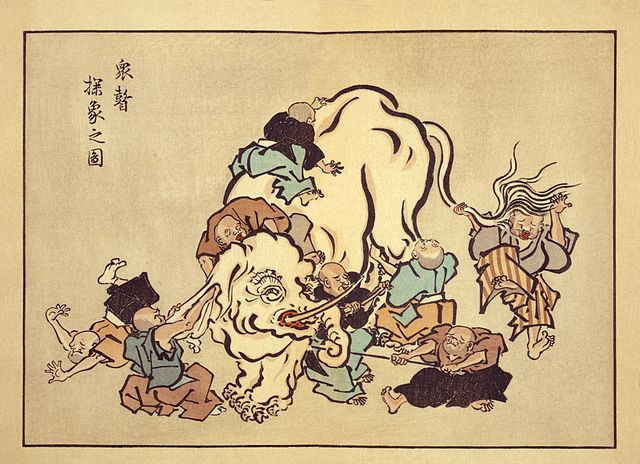
\includegraphics[clip,width=\textwidth]{fig/elephant.jpg}
		\caption{
			かわいそうなゾウ.
			\label{fig:elephant_A}
		}
	\end{subfigure}
	\begin{subfigure}{0.5\textwidth}
		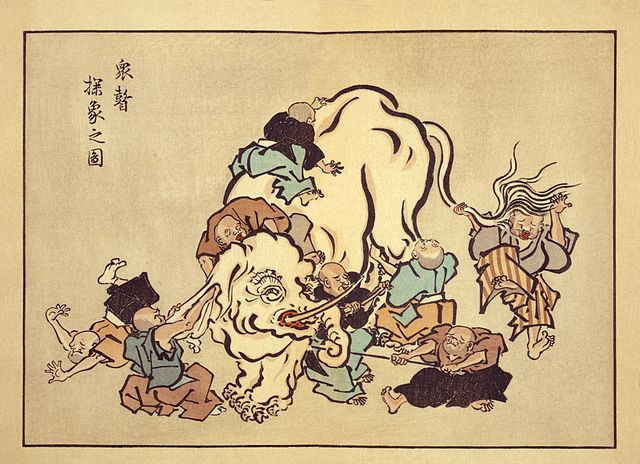
\includegraphics[clip,width=\textwidth]{fig/elephant.jpg}
		\caption{
			きりんさんよりぞうさんがすき.
			\label{fig:elephant_B}
		}
	\end{subfigure}
	\caption{
		群盲象を評す.
		\label{fig:elephant}
	}
\end{figure}

ぞうの卵はおいしいぞう.ぞうの卵はおいしいぞう.ぞうの卵はおいしいぞう.ぞうの卵はおいしいぞう.ぞうの卵はおいしいぞう.ぞうの卵はおいしいぞう.ぞうの卵はおいしいぞう.ぞうの卵はおいしいぞう.ぞうの卵はおいしいぞう.ぞうの卵はおいしいぞう.ぞうの卵はおいしいぞう.ぞうの卵はおいしいぞう.ぞうの卵はおいしいぞう.ぞうの卵はおいしいぞう.ぞうの卵はおいしいぞう.ぞうの卵はおいしいぞう.ぞうの卵はおいしいぞう.ぞうの卵はおいしいぞう.ぞうの卵はおいしいぞう.ぞうの卵はおいしいぞう.ぞうの卵はおいしいぞう.ぞうの卵はおいしいぞう.ぞうの卵はおいしいぞう(\ref{fig:elephant_A,fig:elephant_B}).

\subparagraph{手法1}
ぞうの卵はおいしいぞう.ぞうの卵はおいしいぞう.ぞうの卵はおいしいぞう.ぞうの卵はおいしいぞう.ぞうの卵はおいしいぞう.ぞうの卵はおいしいぞう.ぞうの卵はおいしいぞう.ぞうの卵はおいしいぞう.ぞうの卵はおいしいぞう.ぞうの卵はおいしいぞう.ぞうの卵はおいしいぞう.ぞうの卵はおいしいぞう.ぞうの卵はおいしいぞう.ぞうの卵はおいしいぞう.ぞうの卵はおいしいぞう.ぞうの卵はおいしいぞう.ぞうの卵はおいしいぞう.ぞうの卵はおいしいぞう.ぞうの卵はおいしいぞう.ぞうの卵はおいしいぞう.

\subparagraph{手法2}
ぞうの卵はおいしいぞう.ぞうの卵はおいしいぞう.ぞうの卵はおいしいぞう.ぞうの卵はおいしいぞう.ぞうの卵はおいしいぞう.ぞうの卵はおいしいぞう.ぞうの卵はおいしいぞう.ぞうの卵はおいしいぞう.ぞうの卵はおいしいぞう.ぞうの卵はおいしいぞう.ぞうの卵はおいしいぞう.ぞうの卵はおいしいぞう.ぞうの卵はおいしいぞう.ぞうの卵はおいしいぞう.

\begin{itemize}
	\item ぞうの卵はおいしいぞう.
	\item ぞうの卵はおいしいぞう.
	\item ぞうの卵はおいしいぞう.
\end{itemize}
\begin{enumerate}
	\item ぞうの卵はおいしいぞう.
	\item ぞうの卵はおいしいぞう.
	\item ぞうの卵はおいしいぞう.
\end{enumerate}

\begin{figure}[t]
	\centering
	
\includegraphics[clip,width=0.5\textwidth]{fig/LaTeX.pdf}
	\caption{
		\LaTeX{}の図.
		\label{fig:latex}
	}
\end{figure}

\section{つぎに}
\begin{table}[t]
	\centering
	\caption{
		価格表.
		\label{tab:egg}
	}
	\begin{tabular}{l|cS[table-format=5.0]} % 5 digit int, 0 digit float.
		\toprule
		名称    &   数量  &   金額 \\
		\midrule
		ネズミの卵   &   1    &   1000 \\
		ゾウの卵   &   2    &   10000 \\
		ごまたまご &	12 & 1000 \\
		\bottomrule
	\end{tabular}
\end{table}

\ref{sec:introduction}でも述べたようにゾウの卵はおいしいぞう(\ref{tab:egg}).ゾウの卵はおいしいぞう.ゾウの卵はおいしいぞう.ゾウの卵はおいしいぞう.ゾウの卵はおいしいぞう.ゾウの卵はおいしいぞう.ゾウの卵はおいしいぞう.ゾウの卵はおいしいぞう.ゾウの卵はおいしいぞう.ゾウの卵はおいしいぞう.ゾウの卵はおいしいぞう.ゾウの卵はおいしいぞう.ゾウの卵はおいしいぞう.ゾウの卵はおいしいぞう.ゾウの卵はおいしいぞう.ゾウの卵はおいしいぞう.ゾウの卵はおいしいぞう.ゾウの卵はおいしいぞう.ゾウの卵はおいしいぞう.ゾウの卵はおいしいぞう.ゾウの卵はおいしいぞう.ゾウの卵はおいしいぞう.ゾウの卵はおいしいぞう.ゾウの卵はおいしいぞう.ゾウの卵はおいしいぞう.ゾウの卵はおいしいぞう.ゾウの卵はおいしいぞう.ゾウの卵はおいしいぞう.ゾウの卵はおいしいぞう.ゾウの卵はおいしいぞう.ゾウの卵はおいしいぞう.ゾウの卵はおいしいぞう.ゾウの卵はおいしいぞう.ゾウの卵はおいしいぞう.ゾウの卵はおいしいぞう.ゾウの卵はおいしいぞう.ゾウの卵はおいしいぞう.ゾウの卵はおいしいぞう.ゾウの卵はおいしいぞう.ゾウの卵はおいしいぞう.ゾウの卵はおいしいぞう.ゾウの卵はおいしいぞう.ゾウの卵はおいしいぞう.ゾウの卵はおいしいぞう.ゾウの卵はおいしいぞう.ゾウの卵はおいしいぞう.ゾウの卵はおいしいぞう.ゾウの卵はおいしいぞう.ゾウの卵はおいしいぞう.ゾウの卵はおいしいぞう.ゾウの卵はおいしいぞう.ゾウの卵はおいしいぞう.ゾウの卵はおいしいぞう.ゾウの卵はおいしいぞう.ゾウの卵はおいしいぞう.ゾウの卵はおいしいぞう.ゾウの卵はおいしいぞう.ゾウの卵はおいしいぞう.ゾウの卵はおいしいぞう.ゾウの卵はおいしいぞう.ゾウの卵はおいしいぞう.ゾウの卵はおいしいぞう.ゾウの卵はおいしいぞう.ゾウの卵はおいしいぞう.ゾウの卵はおいしいぞう.ゾウの卵はおいしいぞう.ゾウの卵はおいしいぞう.ゾウの卵はおいしいぞう.ゾウの卵はおいしいぞう.ゾウの卵はおいしいぞう.ゾウの卵はおいしいぞう.ゾウの卵はおいしいぞう.ゾウの卵はおいしいぞう.ゾウの卵はおいしいぞう.ゾウの卵はおいしいぞう.ゾウの卵はおいしいぞう.

\begin{align}
\label{eq:equation1}
a &= b	\\
&= c	\notag\\
\label{eq:equation2}
&= d.
\end{align}

\begin{equation}
\label{eq:equation3}
\begin{aligned}
a &= b	\\
&= c	\\
&= d.
\end{aligned}
\end{equation}

\begin{equation}
\label{eq:equation4}
|a| =
\begin{cases}
a,  & \text{if $a>0$}\\
-a. & \text{if $a<0$}
\end{cases}
\end{equation}

\citet{110001167075}や\citet{mr1763essay}曰く,\ref{eq:equation1,eq:equation2,eq:equation3}は自明.This document contains English, Română, Español and 日本語. This document contains English, Română, Español and 日本語. This document contains English, Română, Español and 日本語. This document contains English, Română, Español and 日本語. This document contains English, Română, Español and 日本語. This document contains English, Română, Español and 日本語. This document contains English, Română, Español and 日本語. This document contains English, Română, Español and 日本語. This document contains English, Română, Español and 日本語. This document contains English, Română, Español and 日本語. This document contains English, Română, Español and 日本語. This document contains English, Română, Español and 日本語. This document contains English, Română, Español and 日本語.

\begin{algorithm}[t]
    \caption{Calculate $y = x^n$}
    \label{alg:algorithm}
    \begin{algorithmic}[1]
        \Require	$n \geq 0 \vee x \neq 0$
        \Ensure	$y = x^n$
        \State $y \Leftarrow 1$
            \If{$n < 0$}
                \State $X \Leftarrow 1 / x$
                \State $N \Leftarrow -n$
            \Else
                \State $X \Leftarrow x$
                \State $N \Leftarrow n$
            \EndIf
        \While{$N \neq 0$}
            \If{$N$ is even}
                \State $X \Leftarrow X \times X$
                \State $N \Leftarrow N / 2$
            \Else[$N$ is odd]
                \State $y \Leftarrow y \times X$
                \State $N \Leftarrow N - 1$
            \EndIf
        \EndWhile
    \end{algorithmic}
\end{algorithm}

{\footnotesize
    %% reference
    \bibliographystyle{jecon_ips}
    \bibliography{bibliography}

    % If no achievements, comment out the below six commands.
    \makeatletter
    \renewcommand{\@biblabel}[1]{#1)} % [N] -> N)
    \makeatother

    \bibliographystyleachieve{jecon_ips}
    \bibliographyachieve{achievement}
    \nociteachieve{*}
}

\end{document}
